\chapter{Qiskit Code}
\label{appendix:B}

\begin{lstlisting}[language=Python, caption={Forming the Bell state $|\Phi^+\rangle = \frac{1}{\sqrt{2}} (|00\rangle + |11\rangle)$}]
import qiskit
from qiskit import QuantumCircuit
from qiskit_aer import AerSimulator
from qiskit.visualization import plot_histogram
import matplotlib.pyplot as plt 
from IPython.display import display, clear_output
clear_output(wait=True)
%matplotlib inline
#Creates circuit with all qubits initialized to the state |0>
bell_circuit = QuantumCircuit(2, 2)

# Create superposition and entanglement
bell_circuit.h(0)  # Apply Hadamard to qubit 0
bell_circuit.cx(0, 1)  # Entangle with qubit 1 by using CNOT

# Add measurement
bell_circuit.measure([0, 1], [0, 1])
print("Circuit diagram")
display(bell_circuit.draw('mpl', style='bw'))

# Simulate the measurement
result = simulator.run(bell_circuit, shots=1000).result()
counts = result.get_counts()

# Display results
print("\nMeasurement results")
display(plot_histogram(counts, title="Measurement results", bar_labels=True))
plt.close('all')
\end{lstlisting}


\subsubsection{Output:}
\begin{figure}[H]
    \centering
    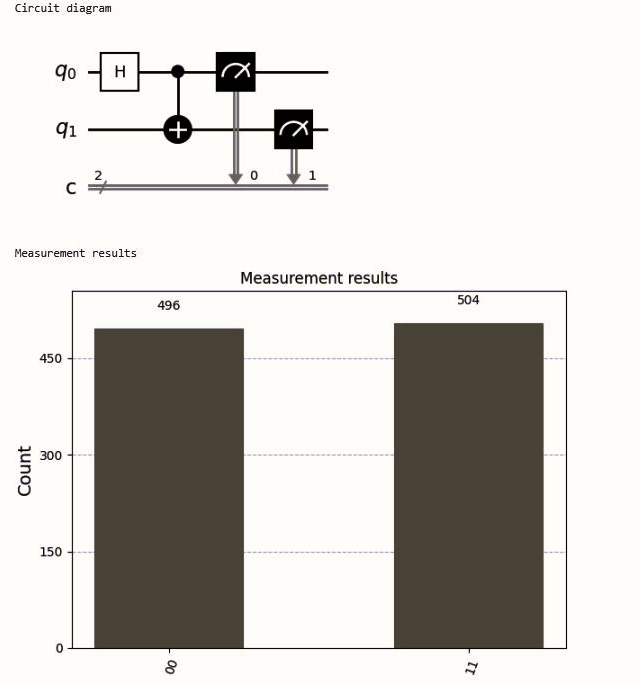
\includegraphics[width=1.1\textwidth]{Bell-state-output.png}
    \label{fig:output1}
\end{figure}
\newpage

\begin{lstlisting}[language=Python, caption={3 Qubit Grover search for the state $|101\rangle$}]
from qiskit import transpile
import numpy as np

target = '101'
iterations = 2  #The optimal number of iterations is pi/4 * sqrt(2^3) which is 
                 #approximately 2

#Creates circuit with all qubits initialized to the state |0>
grover = QuantumCircuit(3, 3)

#Puts all qubits into equal superpositions
grover.h([0, 1, 2])

#Iterative steps
for _ in range(iterations):
    #The oracle operator for |101>
    grover.x(1)  #We need to flip this qubit to convert |101> to |111> as 
                  #the CCZ gate phase just flips |111>
    grover.h(2)
    grover.ccx(0, 1, 2)  #phase flip
    grover.h(2)
    grover.x(1)
    
    #The diffusion operator
    grover.h([0, 1, 2])
    grover.x([0, 1, 2])
    grover.h(2)
    grover.ccx(0, 1, 2)
    grover.h(2)
    grover.x([0, 1, 2])
    grover.h([0, 1, 2])

#Measurement
grover.measure([0, 1, 2], [0, 1, 2])
print("\nCircuit Diagram")
grover.draw('mpl', style='bw', fold=12, cregbundle=False)

#Simulate results
result = AerSimulator().run(grover, shots=1000).result()
counts = result.get_counts()


#Output simulated measurement results
all_states = [format(i, '03b') for i in range(2**3)]
complete_counts = {state: counts.get(state, 0) for state in all_states}
plot_histogram(complete_counts,
               title=f"Measurement results with target |{target}\rangle",
               bar_labels=True)
plt.tight_layout()
plt.show()

print(f"\nProbability of success is {counts.get(target, 0)/1000:.1%}")

\end{lstlisting}

\subsubsection{Output:}
\begin{figure}[H]
    \centering
    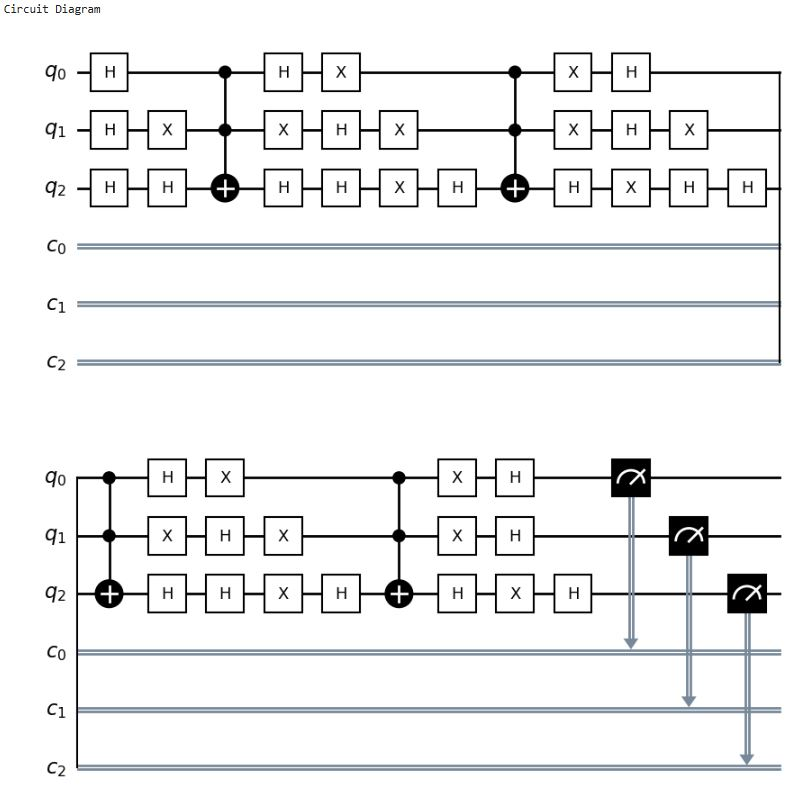
\includegraphics[width=\textwidth]{Grovers-circuit-diagram.png}
    \label{fig:output2}
\end{figure}

\begin{figure}[H]
    \centering
    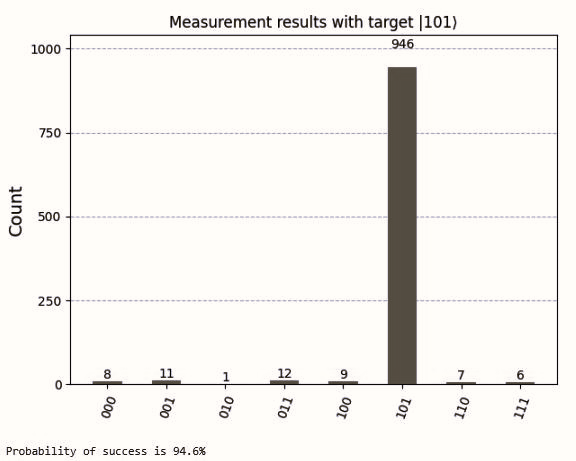
\includegraphics[width=1.0\textwidth]{Grovers-measurement-results.png}
    \label{fig:output3}
\end{figure}